%    Copyright (C)  2011  Santiago Gutierrez Alzate, Sebastian Gomez Gonzalez.

%    Permission is granted to copy, distribute and/or modify this document
%    under the terms of the GNU Free Documentation License, Version 1.3
%    or any later version published by the Free Software Foundation.
%    A copy of the license is included in the section entitled "GNU
%    Free Documentation License" in spanish.

%    Se concede permiso para copiar, distribuir y/o modificar este documento bajo 
%    los términos de la Licencia de Documentación Libre de GNU, Versión 1.3 o 
%    cualquier otra versión posterior publicada por la Free Software Foundation;
%    Una copia de la licencia está incluida en la sección titulada GNU Free
%    Documentation License.


\documentclass[a4paper, 11pt, oneside]{report}

% idioma
\usepackage[utf8]{inputenc}
\usepackage[spanish]{babel}

%tablas
\usepackage{booktabs}

%rotar tablas
\usepackage{rotating}

%color tablas
\usepackage{colortbl}



%espaciado
\usepackage{setspace}
\onehalfspacing
\setlength{\parindent}{0pt}
\setlength{\parskip}{2.0ex plus0.5ex minus0.2ex}


%margenes según n. icontec
\usepackage{vmargin}
\setmarginsrb           { 4.0cm}  % left margin
                        { 3.0cm}  % top margcm
                        { 2.0cm}  % right margcm
                        { 2.0cm}  % bottom margcm
                        {   0pt}  % head height
                        {0.0 cm}  % head sep
                        {   9pt}  % foot height
                        { 1.0cm}  % foot sep

% inserción url's notas de pie.
\usepackage{url}

%gráficos
\usepackage{graphicx}

% Paquetes de la AMS:
\usepackage{amsmath, amsthm, amsfonts}
\addto\captionsspanish{\def\refname{\textsc{Bibliografía}}}

\newcommand\portada{
	\begin{titlepage}
		\begin{center}
			{\large \bf DESARROLLO DE UN SISTEMA PROTOTIPO DE RECONOCIMIENTO DE DÍGITOS USANDO MOMENTOS INVARIANTES }
			\vfill
% 			{\large\bf PRESENTADO POR \par}
			{\large\bf SEBASTIÁN GÓMEZ GONZÁLEZ \par}
			{\large\bf SANTIAGO GUTIERREZ ALZATE \par}
			\vfill
			{\large\bf UNIVERSIDAD TECNOLÓGICA DE PEREIRA  \par}
			{\large\bf FACULTAD DE INGENIERÍAS \par}
			{\large\bf INGENIERÍA DE SISTEMAS Y COMPUTACIÓN \par}
			{\large\bf PEREIRA\par}
			{\large\bf SEPTIEMBRE DE 2010 \par}
		\end{center}
	\end{titlepage}
}

\newcommand\contraportada{
	\begin{titlepage}
		\begin{center}
			{\large \bf DESARROLLO DE UN SISTEMA PROTOTIPO DE RECONOCIMIENTO DE DÍGITOS USANDO MOMENTOS INVARIANTES }
			\vfill
% 			{\large\bf PRESENTADO POR \par}
			{\large\bf SEBASTIÁN GÓMEZ GONZÁLEZ \par}
			{\large\bf SANTIAGO GUTIERREZ ALZATE \par}
			\vfill
			{\large\bf INFORME DE PROYECTO DE GRADO DE PREGRADO\par}
			\vfill
			{\large\bf UNIVERSIDAD TECNOLÓGICA DE PEREIRA  \par}
			{\large\bf FACULTAD DE INGENIERÍAS \par}
			{\large\bf INGENIERÍA DE SISTEMAS Y COMPUTACIÓN \par}
			{\large\bf PEREIRA\par}
			{\large\bf SEPTIEMBRE DE 2010 \par}
		\end{center}
	\end{titlepage}
}

\graphicspath{./diagrams/}

\begin{document}
\portada
\contraportada

\tableofcontents

\chapter{Introducción}

\section{Descripción del problema}

\section{Justificación del proyecto}

\chapter{Métodos estadísticos para la clasificación}

\section{Introducción}

Los métodos de aprendizaje de máquinas, sean de clasificación o de regresión, tienen en común que buscan extraer un modelo que explique un cierto comportamiento de una muestra tomada, para luego generalizar y estimar este comportamiento a cualquier otro elemento de una población. En el caso específico de la clasificación, lo que se busca es que este modelo permita asignar una instancia de la población a alguna de las clases\footnote{ALPAYDIN, Ethem. Introduction to Machine Learning. Estados Unidos: MIT Press, 2004}. En otras palabras, lo que se busca en la clasificación es aprender a clasificar en base a ejemplos.

\begin{figure}[htb]
\begin{center}
\leavevmode
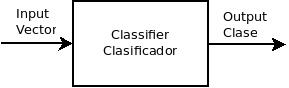
\includegraphics[width=5cm]{diagrams/classifier1.jpg}
\end{center}
\caption{Modelo general de clasificador}
\label{fig:classif1}
\end{figure}

En la figura \ref{fig:classif1} se ve el esquema general de un algoritmo clasificador. Donde lo que se encuentra en la caja ``clasificador'' es el modelo que se va a usar para clasificar. Entonces uno de los problemas que hay que resolver antes de proceder a la clasificación es encontrar un modelo que pueda aproximar lo mejor posible la realidad del problema que se quiere atacar. Varios autores han especificado que hasta el momento no se a encontrado un modelo que se ajuste de la mejor manera a todos los problemas, a esto le han llamado {\it ``no free lunch theorem''}; es español esto traduciría ``teorema no hay almuezo gratis''. En algo si concuerdan la mayoría de investigadores, y es en que si varios modelos funcionan bien se debe escojer el mas sencillo de ellos. Esta observación se desprende del principio filosofico conocido como la navaja de Ockham, propuesto por Guillermo de Ockham (1280-1349), y segun el cual ``cuando dos teorías en igualdad de condiciones tienen las mismas consecuencias, la teoría más simple tiene más probabilidades de ser correcta que la compleja'' \footnote{Robert Audi, ed. Ockham's razor. The Cambridge Dictionary of Philosophy (2nd Edition). Cambridge University Press}. Este principio se aplica en muchos campos, y para el caso del aprendizaje de máquinas tiene especial sentido, ya que usualmente los modelos más sencillos son más fáciles de entrenar, de comprender y sobre todo de depurar.

\subsection{El aprendizaje de máquinas}

Con los avances en las tecnologías de computo, la sociedad tiene la posibilidad de almacenar grandes cantidades de información. Por ejemplo las cadenas de supermercado poseen grandes volumenes de información de sus ventas y las entidades financieras poseen la información crediticia de sus clientes. Para los supermercados es muy útil saber que personas compran ciertos tipos de productos y con que periodicidad, y para las entidades financieras es útil saber que personas son de mayor y menor riesgo para darle un crédito.\newline

Si, por ejemplo, supieramos con exactitud como establecer si una persona es de riesgo o no para una central de crédito dados sus datos financieros, no necesitaríamos utilizar
aprendizaje de máquinas; podríamos simplemente escribir las reglas que determinan si una persona es de riesgo o no en el código. Pero dado que muchas veces no se conocen estas reglas, lo que se busca en el aprendizaje de máquinas es extraer esta información de los datos.\newline

Alpaydin indica que las personas usualmente sabemos que existen procesos que explican los datos que observamos. Por ejemplo, en el caso del supermercado, el comportamiento de los clientes no es completamente aleatorio; por tanto, se espera encontrar algunos patrones en los datos. Aunque este autor indica que muchas veces no es posible identificar el modelo completamente, usualmente se puede construir una buena aproximación. Este es el nicho de trabajo del aprendizaje de máquinas, pues esta aproximación puede ser útil para encontrar patrones en el problema estudiado o para hacer estimaciones de datos futuros asumiendo que en el futuro los datos van a comportarse de una manera similar a como se comportaron en el pasado.

\section{Algunos algoritmos de clasificación}

Como se indicó en la sección anterior, no hay ningun algoritmo que sea la mejor elección para todo tipo de problemas. En esta sección se pretende presentar algunos de los algoritmos o modelos de aprendizaje de máquinas sin ahondar en cada uno de ellos, solo se pretende exponer brevemente de que se tratan y cuales son sus ventajas y desventajas.

\subsection{Árboles de decisión}

Un árbol de decisión es un modelo utilizado principalmente para clasificación. Como su nombre lo dice, el modelo sigue una estructura de árbol, donde los nodos no terminales son condiciones sobre las variables de entrada y los nodos terminales o nodos hoja, son las clases.

\begin{figure}[htb]
\begin{center}
\leavevmode
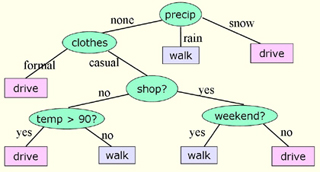
\includegraphics[width=7cm]{img/decisiontree.jpg}
\end{center}
\caption{Ejemplo de árbol de decisión, tomado de MIT OpenCourseware.}
\label{fig:decisionTree}
\end{figure}

En la figura \ref{fig:decisionTree}, se puede ver un ejemplo de un árbol de decisión \footnote{Tomado de ``http://ocw.mit.edu/courses/electrical-engineering-and-computer-science/6-034-artificial-intelligence-spring-2005/'', 12 de Marzo de 2011}. Se puede observar como dependiendo del valor de las variables en cada nodo no terminal, se 
escoje un camino diferente, realizando así un proceso de clasificación. En ese ejemplo, las clases son ``caminar'' y ``conducir''. Es posible examinar el proceso de desición
que se utilizo para llegar a estas variables. Naturalmente, existen procesos automáticos para generar árboles como el del ejemplo a partir de un conjunto de datos de entrenamiento.

De los árboles de decisión se puede concluir:

\begin{itemize}
	\item Son fácilmente interpretables por un ser humano.
	\item Si el árbol esta balanceado correctamente, la velocidad de clasificación es alta.
	\item Se debe configurar la profundidad máxima del árbol.
	\item La mayoría de algoritmos existentes para generar árboles de decisión solo permiten condiciones sobre una única variable por nodo. Por lo tanto el poder clasificatorio de los árboles es limitado.
\end{itemize}

\subsection{Métodos estadísticos}

La estadística es uno de los métodos mas antiguos para inferir el comportamiento de una población a través de una muestra, y sin embargo todavía esta vigente. Se profundizará en este tema en las secciones posteriores, así que por ahora solo se mencionan sus ventajas y desventajas.

\begin{itemize}
	\item No necesita configuración, lo único que se debe saber en el método estadístico a-priori es la distribución de probabilidad con la que se va a  aproximar el modelo real.
	\item El modelo estadístico es fácil de interpretar por un humano, aunque no es tan fácil de intepretar como los árboles de decisión.
	\item El poder clasificatorio es mas alto que el de los árboles de desición.
	\item Brinda mucha información, en vez de solo decir a que clase pertenece una instancia, brida la probabilidad de que la instancia pertenezca a todas las clases, con cierta probabilidad.
\end{itemize}
	
\subsection{Redes neuronales artificiales}

Las redes neuronales artificiales son un paradigma de aprendizaje ampliamente tratado en la literatura de la inteligencia artificial. \footnote{ALPAYDIN, Ethem. Introduction to Machine Learning. Estados Unidos: MIT Press, 2004. 415 p.}. Las redes neuronales artificiales (RNA) intentan imitar la naturaleza de la neuronas del cerebro humano. Uno de los modelos más conocidos de redes neuronales son los perceptrones multicapa. En la figura \ref{fig:rna} se puede apreciar la estructura de un perceptrón multicapa.\footnote{Imagen tomada de Wikimedia Commons ``http://upload.wikimedia.org/wikipedia/commons/6/64/RedNeuronalArtificial.png'', 13 de Marzo de 2011)}.

\begin{figure}[htb]
\begin{center}
\leavevmode
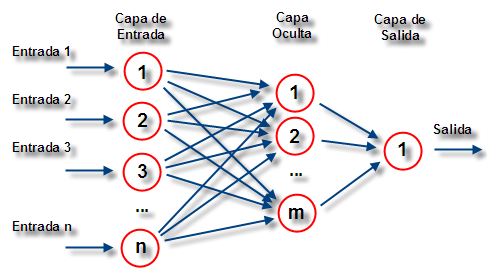
\includegraphics[width=7cm]{img/rna.png}
\end{center}
\caption{Ejemplo de un perceptrón con una capa oculta, tomado de Wikimedia}
\label{fig:rna}
\end{figure}

Cada neurona de un perceptrón multicapa tiene una estructura simple. Cada neurona tiene un vector de datos de entrada $\vec{x}$, un vector de pesos sinápticos $\vec{w}$ y una función de activación $f(x)$. Dado sus entradas, la salida $y$ de una neurona es:

\[y = f(\vec{w}.\vec{x})\]

Las ventajas y desventajas de las redes neuronales son:

\begin{itemize}
	\item El poder clasificatorio de este método es mayor que el de los métodos anteriormente mencionados. Matemáticamente se a demostrado que no exigen ninguna distrubución determinada de los datos, ni separabilidad lineal.
	\item Al igual que el método estadístico, con una función de activación adecuada puede calcular la probabilidad que una instancia pertenezca a cada clase.
	\item Dada la cantidad de parámetros que se pueden configurar, estos algoritmos son muy difíciles de afinar para un problema determinado.
	\item Las redes neuronales son difíciles de interpretar, una vez entrenadas pueden dar buenos o malos resultados, pero es dificil saber cual es el error real o si los resultados se pueden mejorar cambiando los parametros.
\end{itemize}

\section{Algunos elementos de probabilidad}

Un experimento aleatorio es aquel del que no se conoce el resultado con certeza\footnote{Ross, S.M. Introduction to Probability and Statistics for Engineers and Scientists. New York: Wiley 1987.}. El conjunto de todos los posibles resultados se llama espacio muestral $S$, y a cualquier subconjunto de $S$ se le llama evento $E$. Se puede interpretar la probabilidad como una frecuencia: cuando un experimiento es repetido continuamente bajo las mismas condiciones, la proporción de veces que ocurre el evento $E$ en el tiempo se aproxima a un valor constante; a esto lo denotamos $P(E)$ e indica la probabilidad que el evento $E$ ocurra.

\subsection{Probabilidad condicional y el teorema de Bayes}

La probabilidad condicional es la probabilidad de que un evento $A$ ocurra, dado que se conoce la ocurrencia del evento $B$, y se denota $P(A|B)$. La probabilidad condicional se calcula como:

	\begin{equation}\label{condProb}
		P(A|B) = \frac{P(A \cap B)}{P(B)}
	\end{equation}

Al saber que ocurrió el evento $B$, el espacio muestral se reduce al subconjunto $B$. Dado que la intersección es conmutativa, de la equación \eqref{condProb} se obtiene:

\[P(A \cap B) = P(A|B)P(B) = P(B|A)P(A)\]

Y con esto se llega al teorema de Bayes:

	\begin{equation}\label{bayes}
		P(A|B) = \frac{P(B|A)P(A)}{P(B)}
	\end{equation}

Cuando el espacio muestral se compone de varios eventos mutuamente exclusivos $A_i$, es decir, $\cup_{i=1}^{n} A_i = S$ entonces:

\[P(B)=\cup_{i=1}^{n} {A_i \cap B}\]
	\begin{equation}\label{bayesDenominator}
		P(B) = \sum_{i=1}^{n}{P(B|A_i)P(A_i)}
	\end{equation}

Entonces, reemplazando Eq.\eqref{bayesDenominator} en Eq.\eqref{bayes}, tenemos:
	
	\begin{equation}\label{bayes2}
		P(A|B) = \frac{P(B|A)P(A)}{\sum_{i=1}^{n}{P(B|A_i)P(A_i)}}
	\end{equation}
	
\subsection{La esperanza matemática}
Supongamos que se realiza un experimento sobre una variable aleatoria $x$ un número infinito de veces, entonces la esperanza de la variable $x$ es el promedio del valor de $x$ en los infinitos experimentos y se denota $E[x]$ (Que se lee valor esperado de $x$ o esperanza). El concepto de esperanza es importante en la probabilidad porque además de tener usualmente un significado de interés en la variable aleatoria estudiada, se espera que independiente de la distribución de probabilidad que sigue la variable $x$, la esperanza de $x$ converge a un valor constante si las condiciones del experimento no cambian.

\subsection{Distribución de probabilidad}
Una distribución de probabilidad es ...
	
\subsection{La distribución normal}

\section{La distribución normal multivariable}



\chapter{Extracción de características de los caracteres}

\chapter{Diseño, implementación y pruebas del aplicativo}

\chapter{Metodología de la investigación}

\chapter{Conclusiones y resultados}

\section{Primeros resultados}

\section{Mejoras realizadas}

\section{Resultados finales}

\section{Proyectos que se pueden derivar de esta investigación}

\chapter{GNU Free Documentation License}

0. PREÁMBULO

El propósito de esta Licencia es permitir que un manual, libro de texto, u otro documento escrito sea libre en el sentido de libertad: asegurar a todo el mundo la libertad efectiva de copiarlo y redistribuirlo, con o sin modificaciones, de manera comercial o no. En segundo término, esta Licencia proporciona al autor y al editor[2] una manera de obtener reconocimiento por su trabajo, sin que se le considere responsable de las modificaciones realizadas por otros.

Esta Licencia es de tipo copyleft, lo que significa que los trabajos derivados del documento deben a su vez ser libres en el mismo sentido. Complementa la Licencia Pública General de GNU, que es una licencia tipo copyleft diseñada para el software libre.

Hemos diseñado esta Licencia para usarla en manuales de software libre, ya que el software libre necesita documentación libre: un programa libre debe venir con manuales que ofrezcan la mismas libertades que el software. Pero esta licencia no se limita a manuales de software; puede usarse para cualquier texto, sin tener en cuenta su temática o si se publica como libro impreso o no. Recomendamos esta licencia principalmente para trabajos cuyo fin sea instructivo o de referencia.

1. APLICABILIDAD Y DEFINICIONES

Esta Licencia se aplica a cualquier manual u otro trabajo, en cualquier soporte, que contenga una nota del propietario de los derechos de autor que indique que puede ser distribuido bajo los términos de esta Licencia. Tal nota garantiza en cualquier lugar del mundo, sin pago de derechos y sin límite de tiempo, el uso de dicho trabajo según las condiciones aquí estipuladas. En adelante la palabra Documento se referirá a cualquiera de dichos manuales o trabajos. Cualquier persona es un licenciatario y será referido como Usted. Usted acepta la licencia si copia, modifica o distribuye el trabajo de cualquier modo que requiera permiso según la ley de propiedad intelectual.

Una Versión Modificada del Documento significa cualquier trabajo que contenga el Documento o una porción del mismo, ya sea una copia literal o con modificaciones y/o traducciones a otro idioma.

Una Sección Secundaria es un apéndice con título o una sección preliminar del Documento que trata exclusivamente de la relación entre los autores o editores y el tema general del Documento (o temas relacionados) pero que no contiene nada que entre directamente en dicho tema general (por ejemplo, si el Documento es en parte un texto de matemáticas, una Sección Secundaria puede no explicar nada de matemáticas). La relación puede ser una conexión histórica con el tema o temas relacionados, o una opinión legal, comercial, filosófica, ética o política acerca de ellos.

Las Secciones Invariantes son ciertas Secciones Secundarias cuyos títulos son designados como Secciones Invariantes en la nota que indica que el documento es liberado bajo esta Licencia. Si una sección no entra en la definición de Secundaria, no puede designarse como Invariante. El documento puede no tener Secciones Invariantes. Si el Documento no identifica las Secciones Invariantes, es que no las tiene.

Los Textos de Cubierta son ciertos pasajes cortos de texto que se listan como Textos de Cubierta Delantera o Textos de Cubierta Trasera en la nota que indica que el documento es liberado bajo esta Licencia. Un Texto de Cubierta Delantera puede tener como mucho 5 palabras, y uno de Cubierta Trasera puede tener hasta 25 palabras.

Una copia Transparente del Documento, significa una copia para lectura en máquina, representada en un formato cuya especificación está disponible al público en general, apto para que los contenidos puedan ser vistos y editados directamente con editores de texto genéricos o (para imágenes compuestas por puntos) con programas genéricos de manipulación de imágenes o (para dibujos) con algún editor de dibujos ampliamente disponible, y que sea adecuado como entrada para formateadores de texto o para su traducción automática a formatos adecuados para formateadores de texto. Una copia hecha en un formato definido como Transparente, pero cuyo marcaje o ausencia de él haya sido diseñado para impedir o dificultar modificaciones posteriores por parte de los lectores no es Transparente. Un formato de imagen no es Transparente si se usa para una cantidad de texto sustancial. Una copia que no es Transparente se denomina Opaca.

Como ejemplos de formatos adecuados para copias Transparentes están ASCII puro sin marcaje, formato de entrada de Texinfo, formato de entrada de LaTeX, SGML o XML usando una DTD disponible públicamente, y HTML, PostScript o PDF simples, que sigan los estándares y diseñados para que los modifiquen personas. Ejemplos de formatos de imagen transparentes son PNG, XCF y JPG. Los formatos Opacos incluyen formatos propietarios que pueden ser leídos y editados únicamente en procesadores de palabras propietarios, SGML o XML para los cuáles las DTD y/o herramientas de procesamiento no estén ampliamente disponibles, y HTML, PostScript o PDF generados por algunos procesadores de palabras sólo como salida.

La Portada significa, en un libro impreso, la página de título, más las páginas siguientes que sean necesarias para mantener, de manera legible, el material que esta Licencia requiere en la portada. Para trabajos en formatos que no tienen página de portada como tal, Portada significa el texto cercano a la aparición más prominente del título del trabajo, precediendo el comienzo del cuerpo del texto.

El Editor se refiere a cualquier persona o entidad que distribuya copias del Documento a el público.

Una sección Titulada XYZ significa una parte del Documento cuyo título es precisamente XYZ o contiene XYZ entre paréntesis, a continuación de texto que traduce XYZ a otro idioma (aquí XYZ se refiere a nombres de sección específicos mencionados más abajo, como Agradecimientos, Dedicatorias , Aprobaciones o Historia). Conservar el Título de tal sección cuando se modifica el Documento significa que permanece una sección Titulada XYZ según esta definición.[3]

El Documento puede incluir Limitaciones de Garantía cercanas a la nota donde se declara que al Documento se le aplica esta Licencia. Se considera que estas Limitaciones de Garantía están incluidas, por referencia, en la Licencia, pero sólo en cuanto a limitaciones de garantía: cualquier otra implicación que estas Limitaciones de Garantía puedan tener es nula y no tiene efecto en el significado de esta Licencia.

2. COPIA LITERAL

Usted puede copiar y distribuir el Documento en cualquier soporte, sea en forma comercial o no, siempre y cuando esta Licencia, las notas de copyright y la nota que indica que esta Licencia se aplica al Documento se reproduzcan en todas las copias y que usted no añada ninguna otra condición a las expuestas en esta Licencia. Usted no puede usar medidas técnicas para obstruir o controlar la lectura o copia posterior de las copias que usted haga o distribuya. Sin embargo, usted puede aceptar compensación a cambio de las copias. Si distribuye un número suficientemente grande de copias también deberá seguir las condiciones de la sección 3.

Usted también puede prestar copias, bajo las mismas condiciones establecidas anteriormente, y puede exhibir copias públicamente.

3. COPIADO EN CANTIDAD

Si publica copias impresas del Documento (o copias en soportes que tengan normalmente cubiertas impresas) que sobrepasen las 100, y la nota de licencia del Documento exige Textos de Cubierta, debe incluir las copias con cubiertas que lleven en forma clara y legible todos esos Textos de Cubierta: Textos de Cubierta Delantera en la cubierta delantera y Textos de Cubierta Trasera en la cubierta trasera. Ambas cubiertas deben identificarlo a Usted clara y legiblemente como editor de tales copias. La cubierta debe mostrar el título completo con todas las palabras igualmente prominentes y visibles. Además puede añadir otro material en las cubiertas. Las copias con cambios limitados a las cubiertas, siempre que conserven el título del Documento y satisfagan estas condiciones, pueden considerarse como copias literales.

Si los textos requeridos para la cubierta son muy voluminosos para que ajusten legiblemente, debe colocar los primeros (tantos como sea razonable colocar) en la verdadera cubierta y situar el resto en páginas adyacentes.

Si Usted publica o distribuye copias Opacas del Documento cuya cantidad exceda las 100, debe incluir una copia Transparente, que pueda ser leída por una máquina, con cada copia Opaca, o bien mostrar, en cada copia Opaca, una dirección de red donde cualquier usuario de la misma tenga acceso por medio de protocolos públicos y estandarizados a una copia Transparente del Documento completa, sin material adicional. Si usted hace uso de la última opción, deberá tomar las medidas necesarias, cuando comience la distribución de las copias Opacas en cantidad, para asegurar que esta copia Transparente permanecerá accesible en el sitio establecido por lo menos un año después de la última vez que distribuya una copia Opaca de esa edición al público (directamente o a través de sus agentes o distribuidores).

Se solicita, aunque no es requisito, que se ponga en contacto con los autores del Documento antes de redistribuir gran número de copias, para darles la oportunidad de que le proporcionen una versión actualizada del Documento.

4. MODIFICACIONES

Puede copiar y distribuir una Versión Modificada del Documento bajo las condiciones de las secciones 2 y 3 anteriores, siempre que usted libere la Versión Modificada bajo esta misma Licencia, con la Versión Modificada haciendo el rol del Documento, por lo tanto dando licencia de distribución y modificación de la Versión Modificada a quienquiera posea una copia de la misma. Además, debe hacer lo siguiente en la Versión Modificada:

A. Usar en la Portada (y en las cubiertas, si hay alguna) un título distinto al del Documento y de sus versiones anteriores (que deberían, si hay alguna, estar listadas en la sección de Historia del Documento). Puede usar el mismo título de versiones anteriores al original siempre y cuando quien las publicó originalmente otorgue permiso.
B. Listar en la Portada, como autores, una o más personas o entidades responsables de la autoría de las modificaciones de la Versión Modificada, junto con por lo menos cinco de los autores principales del Documento (todos sus autores principales, si hay menos de cinco), a menos que le eximan de tal requisito.
C. Mostrar en la Portada como editor el nombre del editor de la Versión Modificada.
D. Conservar todas las notas de copyright del Documento.
E. Añadir una nota de copyright apropiada a sus modificaciones, adyacente a las otras notas de copyright.
F. Incluir, inmediatamente después de las notas de copyright, una nota de licencia dando el permiso para usar la Versión Modificada bajo los términos de esta Licencia, como se muestra en el Apéndice [Apéndice] al final de este documento.
G. Conservar en esa nota de licencia el listado completo de las Secciones Invariantes y de los Textos de Cubierta que sean requeridos en la nota de Licencia del Documento original.
H. Incluir una copia sin modificación de esta Licencia.
I. Conservar la sección Titulada Historia, conservar su Título y añadirle un elemento que declare al menos el título, el año, los nuevos autores y el editor de la Versión Modificada, tal como figuran en la Portada. Si no hay una sección Titulada Historia en el Documento, crear una estableciendo el título, el año, los autores y el editor del Documento, tal como figuran en su Portada, añadiendo además un elemento describiendo la Versión Modificada, como se estableció en la oración anterior.
J. Conservar la dirección en red, si la hay, dada en el Documento para el acceso público a una copia Transparente del mismo, así como las otras direcciones de red dadas en el Documento para versiones anteriores en las que estuviese basado. Pueden ubicarse en la sección Historia. Se puede omitir la ubicación en red de un trabajo que haya sido publicado por lo menos cuatro años antes que el Documento mismo, o si el editor original de dicha versión da permiso.
K. En cualquier sección Titulada Agradecimientos o Dedicatorias, conservar el Título de la sección y conservar en ella toda la sustancia y el tono de los agradecimientos y/o dedicatorias incluidas por cada contribuyente.
L. Conservar todas las Secciones Invariantes del Documento, sin alterar su texto ni sus títulos. Números de sección o el equivalente no son considerados parte de los títulos de la sección.
M. Borrar cualquier sección titulada Aprobaciones. Tales secciones no pueden estar incluidas en las Versiones Modificadas.
N. No cambiar el título de ninguna sección existente a Aprobaciones ni a uno que entre en conflicto con el de alguna Sección Invariante.
O. Conservar todas las Limitaciones de Garantía.
Si la Versión Modificada incluye secciones o apéndices nuevos que califiquen como Secciones Secundarias y contienen material no copiado del Documento, puede opcionalmente designar algunas o todas esas secciones como invariantes. Para hacerlo, añada sus títulos a la lista de Secciones Invariantes en la nota de licencia de la Versión Modificada. Tales títulos deben ser distintos de cualquier otro título de sección.

Puede añadir una sección titulada Aprobaciones, siempre que contenga únicamente aprobaciones de su Versión Modificada por otras fuentes --por ejemplo, observaciones de peritos o que el texto ha sido aprobado por una organización como la definición oficial de un estándar.

Puede añadir un pasaje de hasta cinco palabras como Texto de Cubierta Delantera y un pasaje de hasta 25 palabras como Texto de Cubierta Trasera en la Versión Modificada. Una entidad solo puede añadir (o hacer que se añada) un pasaje al Texto de Cubierta Delantera y uno al de Cubierta Trasera. Si el Documento ya incluye un textos de cubiertas añadidos previamente por usted o por la misma entidad que usted representa, usted no puede añadir otro; pero puede reemplazar el anterior, con permiso explícito del editor que agregó el texto anterior.

Con esta Licencia ni los autores ni los editores del Documento dan permiso para usar sus nombres para publicidad ni para asegurar o implicar aprobación de cualquier Versión Modificada.

5. COMBINACIÓN DE DOCUMENTOS

Usted puede combinar el Documento con otros documentos liberados bajo esta Licencia, bajo los términos definidos en la sección 4 anterior para versiones modificadas, siempre que incluya en la combinación todas las Secciones Invariantes de todos los documentos originales, sin modificar, listadas todas como Secciones Invariantes del trabajo combinado en su nota de licencia. Así mismo debe incluir la Limitación de Garantía.

El trabajo combinado necesita contener solamente una copia de esta Licencia, y puede reemplazar varias Secciones Invariantes idénticas por una sola copia. Si hay varias Secciones Invariantes con el mismo nombre pero con contenidos diferentes, haga el título de cada una de estas secciones único añadiéndole al final del mismo, entre paréntesis, el nombre del autor o editor original de esa sección, si es conocido, o si no, un número único. Haga el mismo ajuste a los títulos de sección en la lista de Secciones Invariantes de la nota de licencia del trabajo combinado.

En la combinación, debe combinar cualquier sección Titulada Historia de los documentos originales, formando una sección Titulada Historia; de la misma forma combine cualquier sección Titulada Agradecimientos, y cualquier sección Titulada Dedicatorias. Debe borrar todas las secciones tituladas Aprobaciones.

6. COLECCIONES DE DOCUMENTOS

Puede hacer una colección que conste del Documento y de otros documentos liberados bajo esta Licencia, y reemplazar las copias individuales de esta Licencia en todos los documentos por una sola copia que esté incluida en la colección, siempre que siga las reglas de esta Licencia para cada copia literal de cada uno de los documentos en cualquiera de los demás aspectos.

Puede extraer un solo documento de una de tales colecciones y distribuirlo individualmente bajo esta Licencia, siempre que inserte una copia de esta Licencia en el documento extraído, y siga esta Licencia en todos los demás aspectos relativos a la copia literal de dicho documento.

7. AGREGACIÓN CON TRABAJOS INDEPENDIENTES

Una recopilación que conste del Documento o sus derivados y de otros documentos o trabajos separados e independientes, en cualquier soporte de almacenamiento o distribución, se denomina un agregado si el copyright resultante de la compilación no se usa para limitar los derechos de los usuarios de la misma más allá de lo que los de los trabajos individuales permiten. Cuando el Documento se incluye en un agregado, esta Licencia no se aplica a otros trabajos del agregado que no sean en sí mismos derivados del Documento.

Si el requisito de la sección 3 sobre el Texto de Cubierta es aplicable a estas copias del Documento y el Documento es menor que la mitad del agregado entero, los Textos de Cubierta del Documento pueden colocarse en cubiertas que enmarquen solamente el Documento dentro del agregado, o el equivalente electrónico de las cubiertas si el documento está en forma electrónica. En caso contrario deben aparecer en cubiertas impresas enmarcando todo el agregado.

8. TRADUCCIÓN

La Traducción es considerada como un tipo de modificación, por lo que usted puede distribuir traducciones del Documento bajo los términos de la sección 4. El reemplazo las Secciones Invariantes con traducciones requiere permiso especial de los dueños de derecho de autor, pero usted puede añadir traducciones de algunas o todas las Secciones Invariantes a las versiones originales de las mismas. Puede incluir una traducción de esta Licencia, de todas las notas de licencia del documento, así como de las Limitaciones de Garantía, siempre que incluya también la versión en Inglés de esta Licencia y las versiones originales de las notas de licencia y Limitaciones de Garantía. En caso de desacuerdo entre la traducción y la versión original en Inglés de esta Licencia, la nota de licencia o la limitación de garantía, la versión original en Inglés prevalecerá.

Si una sección del Documento está Titulada Agradecimientos, Dedicatorias o Historia el requisito (sección 4) de Conservar su Título (Sección 1) requerirá, típicamente, cambiar su título.

9. TERMINACIÓN

Usted no puede copiar, modificar, sublicenciar o distribuir el Documento salvo por lo permitido expresamente bajo esta Licencia. Cualquier intento en otra manera de copia, modificación, sublicenciamiento, o distribución de él es nulo, y dará por terminados automáticamente sus derechos bajo esa Licencia.

Sin embargo, si usted cesa toda violación a esta Licencia, entonces su licencia proveniente de un titular de copyright queda restaurada (a) provisionalmente, a menos y hasta que el titular del copyright explícita y finalmente termine su licencia, y (b) permanentemente, si el titular del copyright falla en notificarle de la violación por algún medio razonable en un tiempo menor a 60 días después del cese.

Además, su licencia proveniente de un titular del copyright particular queda restaurada permanentemente si el titular del copyright le notifica de la violación por algún método razonable, es la primera vez que usted ha recibido aviso de la violación de esta Licencia (para cualquier trabajo) de ese titular del copyright, y usted remedia la violación en un tiempo menor a 30 días después de recibir dicho aviso.

La terminación de sus derechos bajo ésta sección no termina la licencia de terceros que hayan recibido copias o derechos de usted bajo ésta Licencia. Si sus derechos han sido terminados y no restaurados permanentemente, recibir una copia de alguna parte o el total del mismo material no le da ningún derecho de usarlo.

10. REVISIONES FUTURAS DE ESTA LICENCIA

De vez en cuando la Free Software Foundation puede publicar versiones nuevas y revisadas de la Licencia de Documentación Libre GNU. Tales versiones nuevas serán similares en espíritu a la presente versión, pero pueden diferir en detalles para solucionar nuevos problemas o intereses. Vea http://www.gnu.org/copyleft/.

Cada versión de la Licencia tiene un número de versión que la distingue. Si el Documento especifica que se aplica una versión numerada en particular de esta licencia o cualquier versión posterior, usted tiene la opción de seguir los términos y condiciones de la versión especificada o cualquiera posterior que haya sido publicada (no como borrador) por la Free Software Foundation. Si el Documento no especifica un número de versión de esta Licencia, puede escoger cualquier versión que haya sido publicada (no como borrador) por la Free Software Foundation. Si el Documento especifica que un apoderado puede decidir qué versión futura de esta Licencia puede ser utilizada, esa frase de aceptación del apoderado de una versión le autoriza permanentemente a escoger esa versión para el Documento.

11. Re-Licenciamiento

Un Sitio de Colaboración Masiva Multiautor (o Sitio CMM) significa cualquier servidor World Wide Web que publique trabajos que puedan ser sujetos a copyright y que también provea medios prominentes para que cualquiera pueda editar esos trabajos. Una Wiki pública que cualquiera puede editar es un ejemplo de tal servidor. Una Colaboración Masiva Multiautor (o CMM) contenida en el sitio significa cualquier colección de trabajos que puedan ser sujetos a copyright publicados en el sitio de CMM.

CC-BY-SA significa la licencia Creative Commons Attribution-Share Alike 3.0 (Reconocimiento-Compartir bajo la misma licencia 3.0 de Creative Commons) publicada por Creative Commons Corporation, una corporación sin fines de lucro con base en San Francisco, California, así como versiones futuras copyleft de esa licencia publicada por esa misma organización.

Incorporar significa publicar o re-publicar un Documento, como un todo o parcialmente, como parte de otro Documento.

Un sitio CMM es elegible para re-licenciamiento si es licenciado bajo esta Licencia, y si todos los trabajos que fueron publicados originalmente bajo esta Licencia en algún otro lugar diferente a esta CMM, y subsecuentemente incorporado como un todo o parcialmente a la CMM, (1)no tenía textos de cubierta o secciones invariantes, y (2) fueron incorporados previo a Noviembre 1, 2008.

El operador de un Sitio CMM puede volver a publicar una CMM contenida en el sitio bajo CC-BY-SA en el mismo sitio en cualquier momento antes de Agosto 1, 2009, siempre que la CMM sea elegible para re-licenciamiento.

\end{document}
